\documentclass[11pt]{article}

\usepackage[a4paper,margin=1in]{geometry}
\usepackage{amsmath,amssymb,amsthm,mathtools}
\usepackage{array}
\usepackage{booktabs}
\usepackage{enumitem}
\usepackage{tikz}
\usepackage{physics}
\usepackage{needspace}
\usepackage{xcolor}
\definecolor{courseblue}{RGB}{0,90,150}
\usetikzlibrary{arrows.meta,positioning}

\setlength{\parindent}{0pt}
\setlength{\parskip}{0.75em}

\newcounter{problem}
\newenvironment{problem}{%
    \refstepcounter{problem}%
    \Needspace{7\baselineskip}%
    \par\vspace{0.7em}%
    \noindent\textcolor{courseblue}{\rule{\textwidth}{0.4pt}}%
    \par\vspace{0.5em}%
    \begin{list}{}{%
        \setlength{\leftmargin}{2.3em}%
        \setlength{\labelwidth}{1.8em}%
        \setlength{\labelsep}{0.5em}%
        \setlength{\topsep}{0pt}%
        \setlength{\partopsep}{0pt}%
    }%
    \item[{[\theproblem]}]
}{%
    \end{list}
    \par\vspace{0.5em}
}

\newenvironment{parts}{%
    \begin{enumerate}[label={[\alph*]},leftmargin=2.2em,itemsep=0.65em,topsep=0.65em]
}{%
    \end{enumerate}
}

% Type each solution between \begin{answer} and \end{answer}.
\newenvironment{answer}{%
    \Needspace{4\baselineskip}%
    \par\vspace{0.35em}
    \noindent\textbf{Answer:}\par
}{%
    \par\vspace{0.25em}
}



% The optional style marks the two E_2 edges in the second source graph.
\newcommand{\trianglegraph}[1][]{%
    \begin{tikzpicture}[
        vertex/.style={circle,draw,fill=gray!15,minimum size=6mm,inner sep=0pt},
        line width=0.6pt
    ]
        \node[vertex] (1) at (0,0) {1};
        \node[vertex] (2) at (0,2) {2};
        \node[vertex] (3) at (2,1) {3};
        \node[vertex] (4) at (4,2) {4};
        \node[vertex] (5) at (4,0) {5};
        \node[vertex] (6) at (7,2) {6};
        \node[vertex] (7) at (7,0) {7};
        \draw (1)--(2)--(4)--(6)--(7)--(5)--(1);
        \draw (3)--(4)--(5)--(3);
        \draw (4)--(7);
        \draw[#1] (1)--(3);
        \draw[#1] (2)--(3);
    \end{tikzpicture}%
}

\title{CO250 Assignment 2}
\author{}
\date{September 21--28}

\begin{document}
\maketitle

\begin{problem}
    An art thief has broken into a museum and wants to steal as many art pieces as they can.
    However, they are on their own and can only carry a limited amount of weight. They want to
    steal art totaling as much value as they can. The following is a collection of art pieces that
    they can steal and their weights and their values.

    \begin{center}
    \begin{tabular}{c|*{6}{c}}
        \toprule
        Piece & 1 & 2 & 3 & 4 & 5 & 6 \\
        \midrule
        Weight (kg) & 10 & 15 & 7 & 8 & 5 & 3 \\
        Value (\$) & 50 & 100 & 30 & 50 & 12 & 15 \\
        \bottomrule
    \end{tabular}
    \end{center}

    \begin{parts}
        \Needspace{8\baselineskip}\item Formulate an integer program that that models the thief's situation, assuming that they
        can only hold 30kg of art. Clearly explain your variables, objective function and constraints.
        \begin{answer}
            let $x_i\in\{0,1\}$ be a binary variable representing the choice of taking item $i$. \\
            let $x = (x_1,x_2,x_3,x_4,x_5,x_6)$
            \begin{align*}
                \text{Objective:}\qquad
                    & \max [50,100,30,50,12,15]x \\
                \text{subject to:}\qquad
                    & [10,15,7,8,5,3]x \leq 30\\
                    & x_i \in\{0,1\}\qquad \forall i\in[6].
            \end{align*}
        \end{answer}

        \Needspace{8\baselineskip}\item Suppose that in fact, the art thief has two bags, each of which can hold 15 kg of art. How
        do we need to change the previous integer program to model this change?
        \begin{answer}
            let $x_i\in\{0,1\}$ be a binary variable representing the choice of taking item $i$ in sack 1. 
            let $y_i\in\{0,1\}$ be a binary variable representing the choice of taking item $i$ in sack 2. 
            let $x = (x_1,x_2,x_3,x_4,x_5,x_6)$
            let $y = (y_1,y_2,y_3,y_4,y_5,y_6)$

            \begin{align*}
                \text{Objective:}\qquad
                    & \max [50,100,30,50,12,15](x + y)\\
                \text{subject to:}\qquad
                    & [10,15,7,8,5,3]x \leq 15\\
                    & [10,15,7,8,5,3]y \leq 15\\
                    & x + y \leq \vec{1}\\
                    & x_i \in\{0,1\} \qquad \forall i\in[6]\\
                    & y_i \in\{0,1\} \qquad \forall i\in[6]
            \end{align*}
        \end{answer}
    \end{parts}
\end{problem}

\begin{problem}
    A music venue needs to schedule acts for the week. They operate Friday through Sunday,
    and each day, they schedule one act. There are 4 possible bands that they can schedule, but
    each band has only certain nights they can play. Below is a table that shows which bands are
    available on which nights.

    \begin{center}
    \begin{tabular}{l|ccc}
        & Friday & Saturday & Sunday \\
        \hline
        Band 1 & $\checkmark$ & & $\checkmark$ \\
        Band 2 & & $\checkmark$ & \\
        Band 3 & $\checkmark$ & $\checkmark$ & \\
        Band 4 & & & $\checkmark$
    \end{tabular}
    \end{center}

    \begin{parts}
        \Needspace{8\baselineskip}\item Draw the availability data as a bipartite graph. (A graph $G=(V,E)$ is bipartite if $V$ can
        be partition into two parts $A$ and $B$ such that every edge $e$ in $E$ has exactly one end in $A$
        and one end in $B$.)
        \begin{answer}
            \begin{center}
            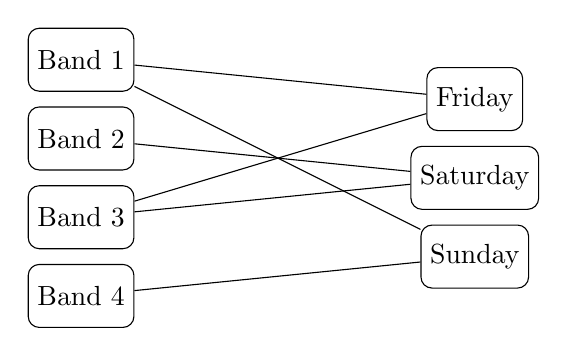
\begin{tikzpicture}[scale=1, every node/.style={draw, rectangle, rounded corners, minimum width=12mm, minimum height=8mm}]
                % Band nodes
                \node (b1) at (0,3) {Band 1};
                \node (b2) at (0,2) {Band 2};
                \node (b3) at (0,1) {Band 3};
                \node (b4) at (0,0) {Band 4};
            
                % Day nodes
                \node (f) at (5,2.5) {Friday};
                \node (s) at (5,1.5) {Saturday};
                \node (u) at (5,0.5) {Sunday};
            
                % Edges
                \draw (b1) -- (f);
                \draw (b1) -- (u);
                \draw (b2) -- (s);
                \draw (b3) -- (f);
                \draw (b3) -- (s);
                \draw (b4) -- (u);
            \end{tikzpicture}
            \end{center}
            \end{answer}

        \Needspace{8\baselineskip}\item What does a valid scheduling correspond to in this bipartite graph? Find and draw a
        valid schedule for this music venue.
        \begin{answer}
            A valid schedule corresponds to a matching of size 3 in the bipartite graph, where every day vertex is incident to exactly one selected edge.
            
            For example, a valid schedule is:
            \[
            \{\,(B_1,\text{Friday}),\ (B_2,\text{Saturday}),\ (B_4,\text{Sunday})\,\}.
            \]
            
            \begin{center}
            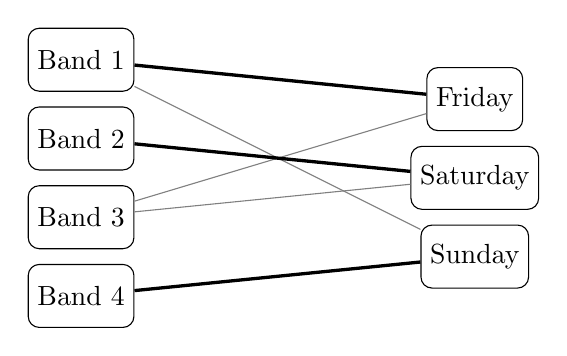
\begin{tikzpicture}[scale=1, every node/.style={draw, rectangle, rounded corners, minimum width=12mm, minimum height=8mm}]
                % Band nodes
                \node (b1) at (0,3) {Band 1};
                \node (b2) at (0,2) {Band 2};
                \node (b3) at (0,1) {Band 3};
                \node (b4) at (0,0) {Band 4};
            
                % Day nodes
                \node (f) at (5,2.5) {Friday};
                \node (s) at (5,1.5) {Saturday};
                \node (u) at (5,0.5) {Sunday};
            
                % Unselected availability edges
                \draw[gray] (b1) -- (u);
                \draw[gray] (b3) -- (f);
                \draw[gray] (b3) -- (s);
            
                % Selected schedule edges
                \draw[very thick] (b1) -- (f);
                \draw[very thick] (b2) -- (s);
                \draw[very thick] (b4) -- (u);
            \end{tikzpicture}
            \end{center}
            \end{answer}

        \Needspace{12\baselineskip}\item Write down an integer program that solves this problem. The integer program should be
        of the form
        \[
        \begin{aligned}
            \min \quad & c^{\mathsf{T}}x \\
            \text{such that}\quad & Ax\leq b \\
            & 1\geq x\geq 0 \\
            & x\in\mathbb{Z}^k,
        \end{aligned}
        \]
        where $A$ is a matrix and $c$ is a vector, and $k$ is an integer.
        \begin{answer}
            Let
            \[
            x =
            \begin{bmatrix}
            x_{1F} \\
            x_{1Su} \\
            x_{2Sa} \\
            x_{3F} \\
            x_{3Sa} \\
            x_{4Su}
            \end{bmatrix},
            \]
            where $x_{ij}=1$ if the edge $\{i,j\}$ is chosen in the matching,
            and $x_{ij}=0$ otherwise.
            
            We want to maximize the number of selected edges. Since the required
            form uses a minimization problem, we equivalently minimize the negative
            of the number of selected edges. Thus,
            \[
            c =
            \begin{bmatrix}
            -1\\
            -1\\
            -1\\
            -1\\
            -1\\
            -1
            \end{bmatrix}.
            \]
            
            For each vertex, at most one incident edge may be selected. Hence,
            \[
            A =
            \begin{bmatrix}
            1 & 1 & 0 & 0 & 0 & 0 \\
            0 & 0 & 1 & 0 & 0 & 0 \\
            0 & 0 & 0 & 1 & 1 & 0 \\
            0 & 0 & 0 & 0 & 0 & 1 \\
            1 & 0 & 0 & 1 & 0 & 0 \\
            0 & 0 & 1 & 0 & 1 & 0 \\
            0 & 1 & 0 & 0 & 0 & 1
            \end{bmatrix},
            \qquad
            b =
            \begin{bmatrix}
            1\\
            1\\
            1\\
            1\\
            1\\
            1\\
            1
            \end{bmatrix}.
            \]
            
            Therefore, the integer program is
            \[
            \begin{aligned}
                \min \quad & c^{\mathsf T}x \\
                \text{such that}\quad
                    & Ax \leq b, \\
                    & 1 \geq x \geq 0, \\
                    & x \in \mathbb{Z}^6.
            \end{aligned}
            \]
            \end{answer}
    \end{parts}
\end{problem}

\begin{problem}
    We are given a graph $G$ representing a network. A \emph{triangle} in the graph is a set of three
    distinct nodes $i,j,k$ such that all pairs $ij,jk,ik$ are edges in $G$. Our goal is to pick as many
    triangles as possible so that no pair of triangles share an edge. Note that triangles are allowed
    to share nodes (triangles represent self-contained subnetworks that cannot share communication
    lines with other subnetworks). For the graph below the set of triangles $\{123,345,467\}$
    would be a feasible solution; the set of triangles $\{123,135\}$ would not be a feasible solution (the
    edge $13$ is used by two triangles).

    \begin{parts}
        \Needspace{17\baselineskip}\item Formulate the above-mentioned problem as an IP for the following graph $G$.
        \begin{center}
            \trianglegraph
        \end{center}
        \emph{Hint: First, list all the triangles in $G$. Then introduce a binary variable for each triangle.
        Then, for each edge $ij$ in the graph, write a constraint that ``says:'' among the triangles
        which use this edge $ij$ we may pick at most one of them.}
        \begin{answer}
            The triangles in $G$ are
            \[
            T=\{123,234,135,345,457,467\}.
            \]
            
            For each triangle $ijk\in T$, let
            \[
            x_{ijk}=
            \begin{cases}
            1, & \text{if triangle $ijk$ is selected},\\
            0, & \text{otherwise}.
            \end{cases}
            \]
            
            We want to select as many triangles as possible. Thus,
            \[
            \begin{aligned}
                \max \quad
                    & x_{123}+x_{234}+x_{135}+x_{345}+x_{457}+x_{467}\\
                \text{subject to}\quad
                    & x_{123}+x_{135}\leq 1,\\
                    & x_{123}+x_{234}\leq 1,\\
                    & x_{135}+x_{345}\leq 1,\\
                    & x_{234}+x_{345}\leq 1,\\
                    & x_{457}+x_{345}\leq 1,\\
                    & x_{457}+x_{467}\leq 1,\\
                    & x_{123},x_{234},x_{135},x_{345},x_{457},x_{467}\in\{0,1\}.
            \end{aligned}
            \]
            \end{answer}

        \Needspace{8\baselineskip}\item Now, suppose we are given an arbitrary graph $G$ with node set $V$ and edge set $E$. Let $T$
        denote the set of triangles in $G$. Write down your IP model for this general set-up.
        \begin{answer}
            For every triangle $t\in T$, let
            \[
            x_t =
            \begin{cases}
            1, & \text{if triangle $t$ is selected},\\
            0, & \text{otherwise}.
            \end{cases}
            \]
            
            We want to select as many triangles as possible, so the objective is
            \[
            \max \sum_{t\in T} x_t.
            \]
            
            For each edge $e\in E$, at most one selected triangle may contain that edge.
            Thus, for every $e\in E$,
            \[
            \sum_{\substack{t\in T\\ e\in t}} x_t \leq 1.
            \]
            
            Therefore, the integer program is
            \[
            \begin{aligned}
                \max \quad & \sum_{t\in T} x_t\\
                \text{subject to}\quad
                    & \sum_{\substack{t\in T\\ e\in t}} x_t \leq 1
                    && \forall e\in E,\\
                    & x_t\in\{0,1\}
                    && \forall t\in T.
            \end{aligned}
            \]
            \end{answer}

        \Needspace{18\baselineskip}\item Next consider a graph $G$ whose edge set $E$ is made up from two types of edges $E_1$ and
        $E_2$. In these graphs the edges in $E_1$ have the same rule as before; but, the edges in $E_2$
        can be used by at most two triangles (instead of at most one). For the graph below where
        $E_2:=\{13,23\}$, formulate the new problem as an IP. Your formulation should be easily
        generalizable to any graph $G$.
        \begin{center}
            \trianglegraph[double,double distance=1pt]
        \end{center}
        \begin{answer}
            For every triangle $t\in T$, let $x_t\in\{0,1\}$ indicate whether
            triangle $t$ is selected.
            
            \[
            \begin{aligned}
                \max \quad & \sum_{t\in T} x_t\\
                \text{subject to}\quad
                    & \sum_{\substack{t\in T\\ e\in t}} x_t \leq 1
                    && \forall e\in E_1,\\
                    & \sum_{\substack{t\in T\\ e\in t}} x_t \leq 2
                    && \forall e\in E_2,\\
                    & x_t\in\{0,1\}
                    && \forall t\in T.
            \end{aligned}
            \]
            \end{answer}
    \end{parts}
\end{problem}

\end{document}
